\documentclass[a4paper,titlepage,11pt]{ltjsarticle}
\usepackage{graphicx}
\usepackage{amssymb}
\usepackage{here}
\begin{document}
%%タイトル
\title{システム開発入門\\レポート課題2}
\author{2022531033 関川謙人}
\maketitle

%%%%%%一章%%%%%%%%
\section{目的}
この授業の後半部分の目的は、ソフトウェアにより設計したプログラムを実際にハードウェアに
実装することで、身近な機器の仕組みについて理解することにあると考えられる。また実際に
自分で機会を設計することで、各人の独創性を生かし、モノづくりのやり方の大枠を捉えることが
この授業の意義であると考える。
\section{課題について}
\subsection{課題1}
%%%%%%%%課題2 フロントパネル%%%%%%%%%%%%%%%%
\begin{figure}[H]
  \begin{center}
    \includegraphics[width=100mm]{kadai1.pdf}
    \caption{課題1 Labview画面}
  \end{center}
\end{figure}
%%%%%%%%%%%%%%%%%%%%%%
課題1の実現方法は、上図のようにLabviewの画面上でスイッチを実装し、
画面上のLEDにBool関数を入力、またDigital Writeにスイッチで生成した
Bool値を入力することで実現できる。
\subsection{課題2}
%%%%%%%%課題2 フロントパネル%%%%%%%%%%%%%%%%
\begin{figure}[H]
  \begin{center}
    \includegraphics[width=100mm]{patern_b.pdf}
    \caption{課題2 フロントパネル}
  \end{center}
\end{figure}
%%%%%%%%%%%%%%%%%%%%%%
このフロントパネルにおいて、digital readでブレボ
上の電圧を読み取り、その結果となるBool値をdigital Writeに
渡し、bool値によって実行の可否を判断する仕組みとなっている。
スイッチが押された場合、電圧がGNDに流れて判定部分の電圧がゼロになるため
digital readの値はNoとなるが、しかしスイッチを押したときにDigital Write
が作動してLEDが光るようにしたいので間にNotを挟む必要がある。
%%%%%%%%%%%ハード面%%%%%%%%%%%%%%
\begin{figure}[H]
  \begin{center}
    \includegraphics[width=100mm]{patern_h.pdf}
    \caption{課題2の電気設計}
  \end{center}
\end{figure}
%%%%%%%%%%%%%%%%%%%%%%%%%%%%%
上図のように、ブレボ上のスイッチを押下すると、ブレボ上のLED
と同時にフロントパネル上のLEDも反応するようになっている。
配線面ではD2、D4からLEDに出力し、D5、D7で抵抗とスイッチの
間の電圧を読み取ることができるようにしている。
\subsection{課題3}
%%%%%%%%%%%%%%%%%%%%
\begin{figure}[H]
  \begin{center}
    \includegraphics[width=100mm]{kadai3_b.pdf}
    \caption{課題3 ブロックダイアグラム}
  \end{center}
\end{figure}
%%%%%%%%%%%%%%%%%%%%%
課題3のブロックダイアグラムにおいて,
初めに読み取るスイッチをS1,その次に読み取るスイッチをS2とし、
S1によって動く入力制御部分をループ1,S2によって動く部分をループ2
とする。
最初にDigital readでS1が押下されているかを判断し、サーボモータ
ーへの入力を制御する部分に渡す。次にS2が押下されているかを確認
し、同様にする。次に入力制御部分からサーボモーターに数値を渡し、
サーボモーターを動かす。

入力制御部分においてはS1から渡された
Bool値がFalse(S1が押下されている)限り、ループ1は動作する。
ループ1においては外から入力されたデフォルト値1500に1を足し続ける。
サーボモーターに渡す値$n$が2500に達したときもしくはスイッチが押下されなくなったときに
ループ1はストップする。そしてループ2に$n$を渡す。ループ2も開始、
終了条件はループ1とほぼ同じであるが、ループ2は$n$から1を
引き続け、$n$が500に達したときに終了する。最終的に$n$の値を
サーボモーターに渡す。
%%%%%フロントパネル%%%%%%
\begin{figure}[H]
  \begin{center}
    \includegraphics[width=100mm]{kadai3_f.pdf}
    \caption{課題3 フロントパネル}
  \end{center}
\end{figure}
%%%%%%ハード構造%%%%%%
\begin{figure}[H]
  \begin{center}
    \includegraphics[width=100mm]{kadai3_h.pdf}
    \caption{課題3の電気構造}
  \end{center}
\end{figure}
%%%%%%%%%%%%%%%%%%%%%%
上の実験画像から、スイッチを押したとき、サーボモーターの振り向き角が変化
していることがわかる。

\section{実験方法:自由課題;ポケモンタイプ相性チェッカー}
このセクションでは、タイプ相性判定部分、攻撃、防御側タイプ選択部分、
全体のシステム制御部分の三つに分けてプログラムを説明する。
\begin{figure}[H]
  \begin{center}
    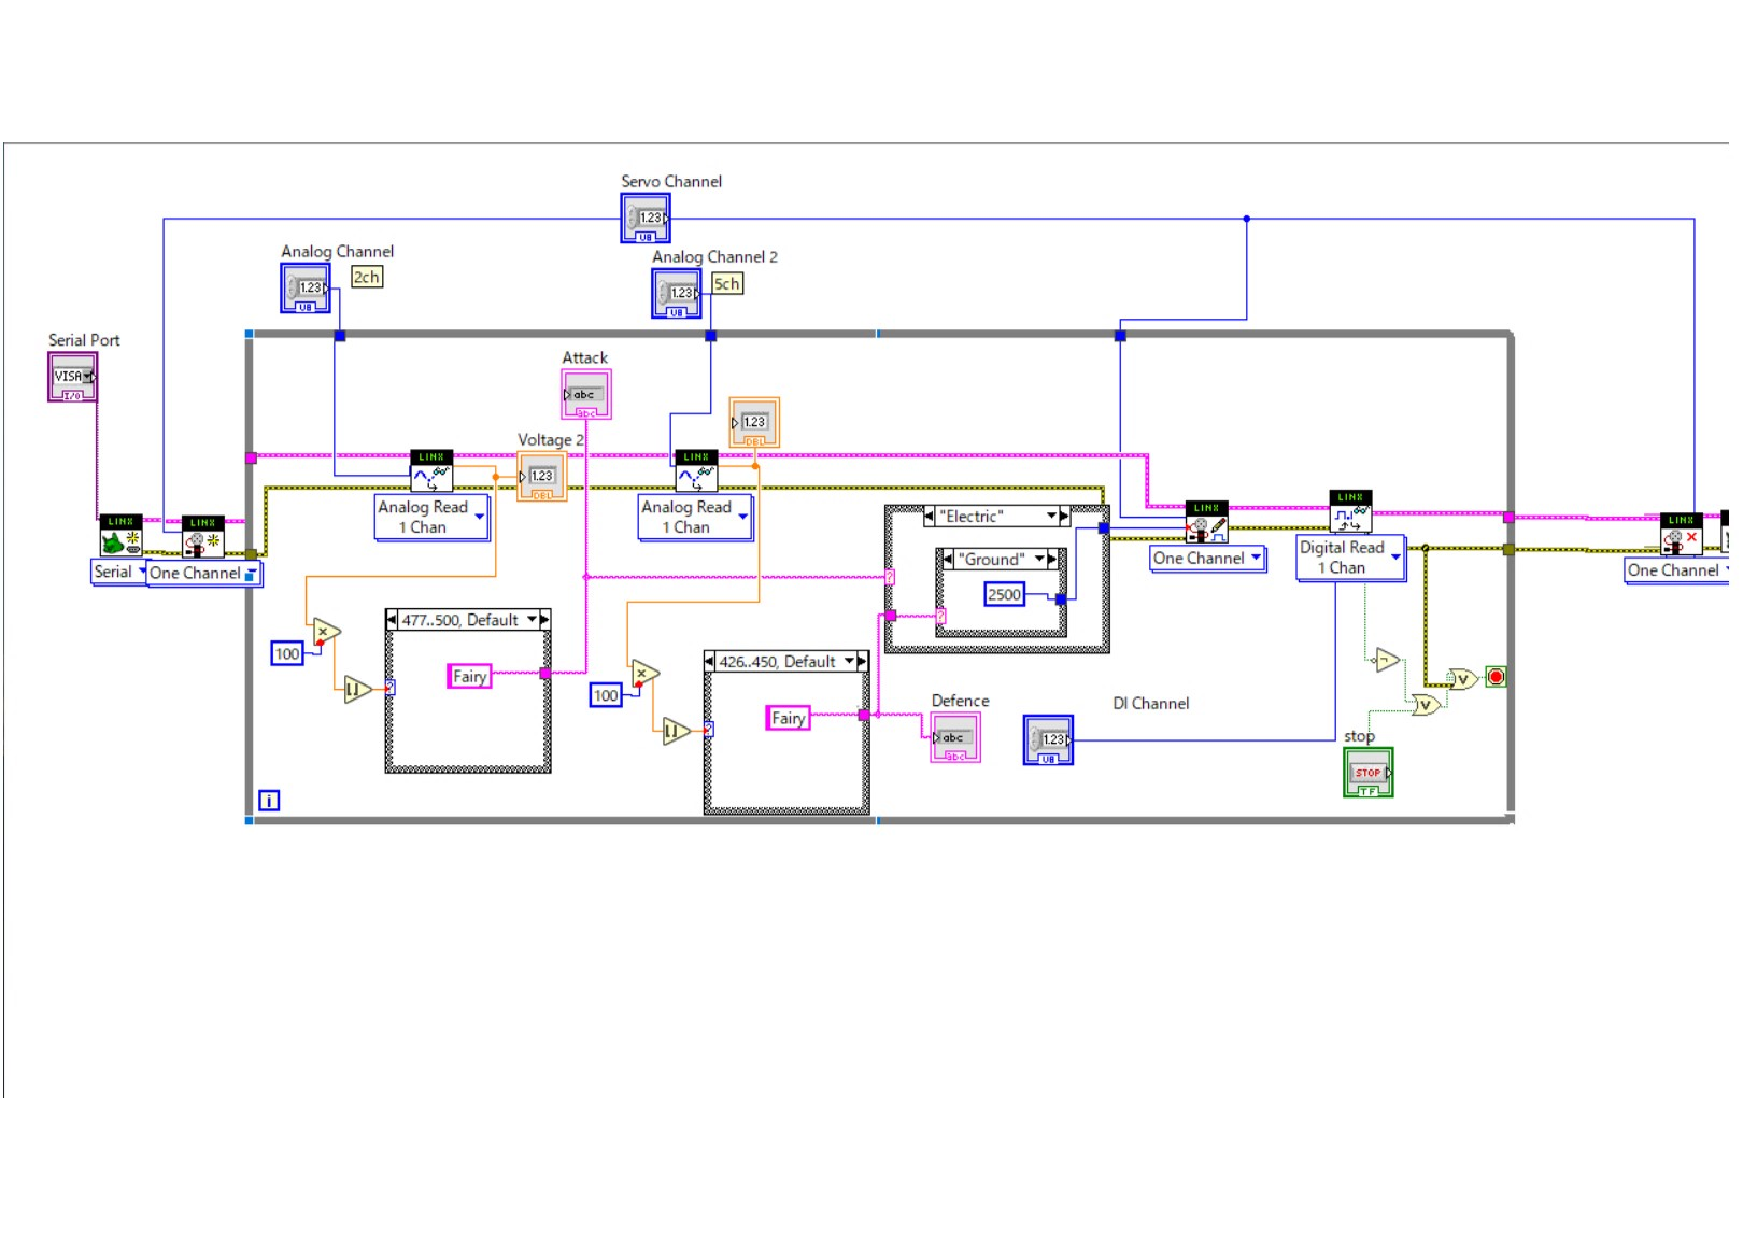
\includegraphics[width=150mm]{selfmade_b.pdf}
    \caption{ブロックダイアグラムの全体像}
  \end{center}
\end{figure}
\begin{figure}[H]
  \begin{center}
    \includegraphics[width=100mm]{selfmade_h1.pdf}
    \caption{ハードウェアにおける全体像}
  \end{center}
\end{figure}
\subsection{全体のシステム制御}
上図はそれぞれ相性チェッカーの全体像となっている。
プログラムとハードウェアの動きを簡略化した図を下に示す。
\begin{figure}[H]
  \begin{center}
    \includegraphics[width=100mm]{hardtosoft.pdf}
    \caption{全体の動き}
  \end{center}
\end{figure}
このように、まずLabviewのLINXおよびopen servoで制御装置、およびサーボモーターとの接続を確立する。
その後可変抵抗によってAnalog readへ流す電圧を調整してLabviewへ渡す。その電圧をもとに攻撃および
防御側のタイプ選択部分を通してタイプを選択し、タイプ相性判定部分へ渡す。タイプ相性判定部分から
サーボモーターへ回転角を指示する。そしてサーボモーターで相性補正を表示する。また物理的なストップ
ボタン、Labview画面上のストップボタンの両方でWhileループを止めることができるようになっている。
whileループが止まったあと、Servo closeとLINX closeで接続を切断し、制御を終える。
\subsection{サーボモーター}
\begin{figure}[H]
  \begin{center}
    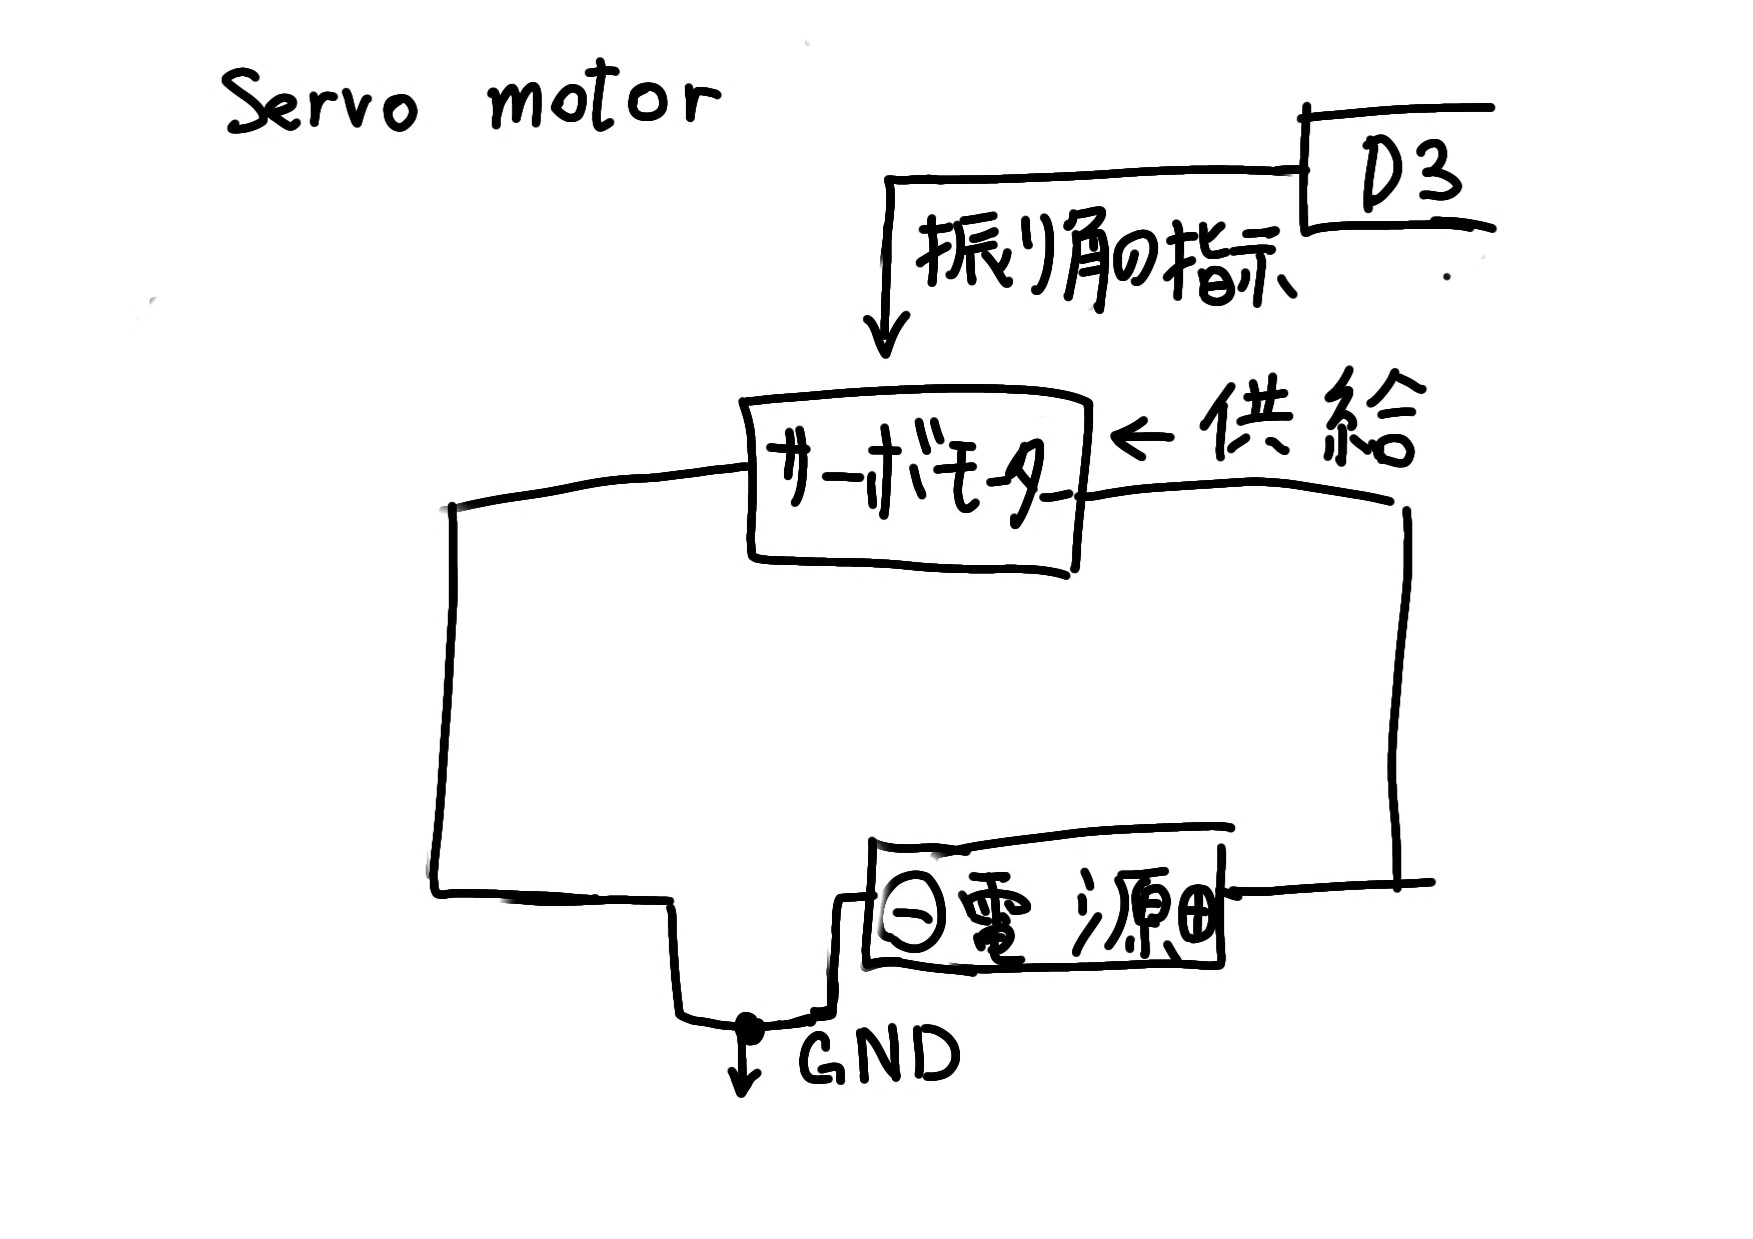
\includegraphics[width=100mm]{servo_h.pdf}
    \caption{サーボモーター周辺の回路図}
  \end{center}
\end{figure}
  Labview上のDigital Servoから渡された回転角の指示を、Digitalを通して受け取る。
  今回はD3にその役割を与えた。また外部電源から電気を受け取り、その電気でモータを
  動かし、最終的に電流はGNDへ流れる。
\subsection{タイプ相性表}
\begin{figure}[H]
  \begin{center}
    \includegraphics[width=100mm]{typechart.pdf}
    \caption{ポケモンタイプ相性表\cite{typechart}}
  \end{center}
\end{figure}
次にタイプ相性判定部分について説明する。参考にしたタイプ相性は以上の図の通りである。
また以下の図はタイプ相性とポケモンのゲーム上のダメージ倍率、サーボモーターに渡す値の関係性を表す表に
なっている。

%%%%表%%%%%%%%%
\begin{tabular}{|c|c|c|}\hline
  相性 & ダメージ倍率 & サーボモーター値 \\ \hline
  効果抜群 & 2 & 500 \\ \hline
  等倍 & 1 & 1175 \\ \hline
  今一つ & 1/2 & 1825 \\ \hline
  効果なし & 0 & 2500 \\ \hline
\end{tabular}
%%%%表ここまで%%%%

以上の二つの表をケースストラクチャを利用してLabviewに落とし込んだ。
\begin{figure}[H]
  \begin{center}
    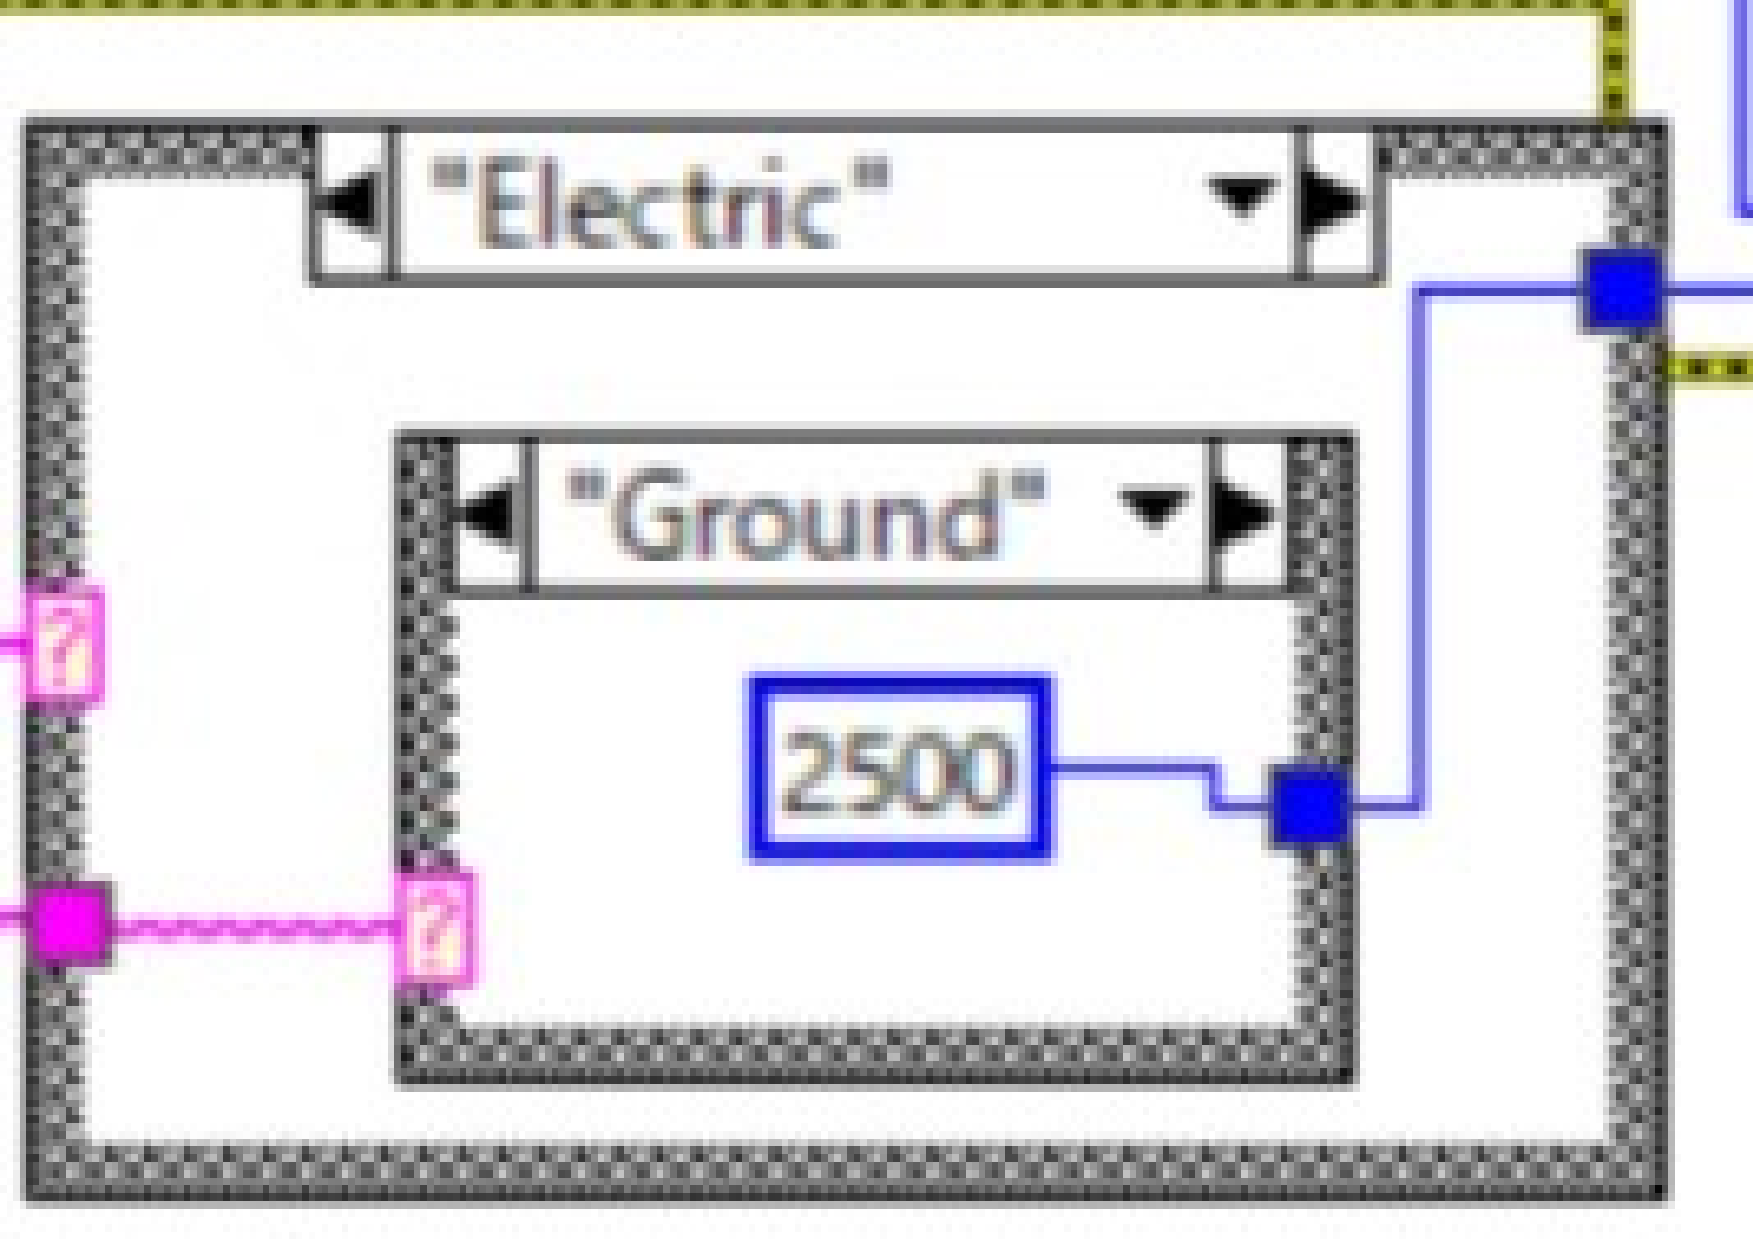
\includegraphics[width=100mm]{typechart_lab.pdf}
    \caption{タイプ相性の実装}
  \end{center}
\end{figure}
ケースストラクチャを二重に組み合わせることで特定の組み合わせで特定の回転角を指定する。
このことで二つのタイプの相性を実装することができている。ケースストラクチャの条件分岐にはタイプのString値を渡している。
また実装における効率化のために、一番多い相性である「等倍」の概念は、Defaltストラクチャを利用して実装している。
\subsection{可変抵抗によるタイプ選択}
可変抵抗のつまみを回すことでタイプのString値を指定することができる装置について。
\begin{figure}[H]
  \begin{center}
    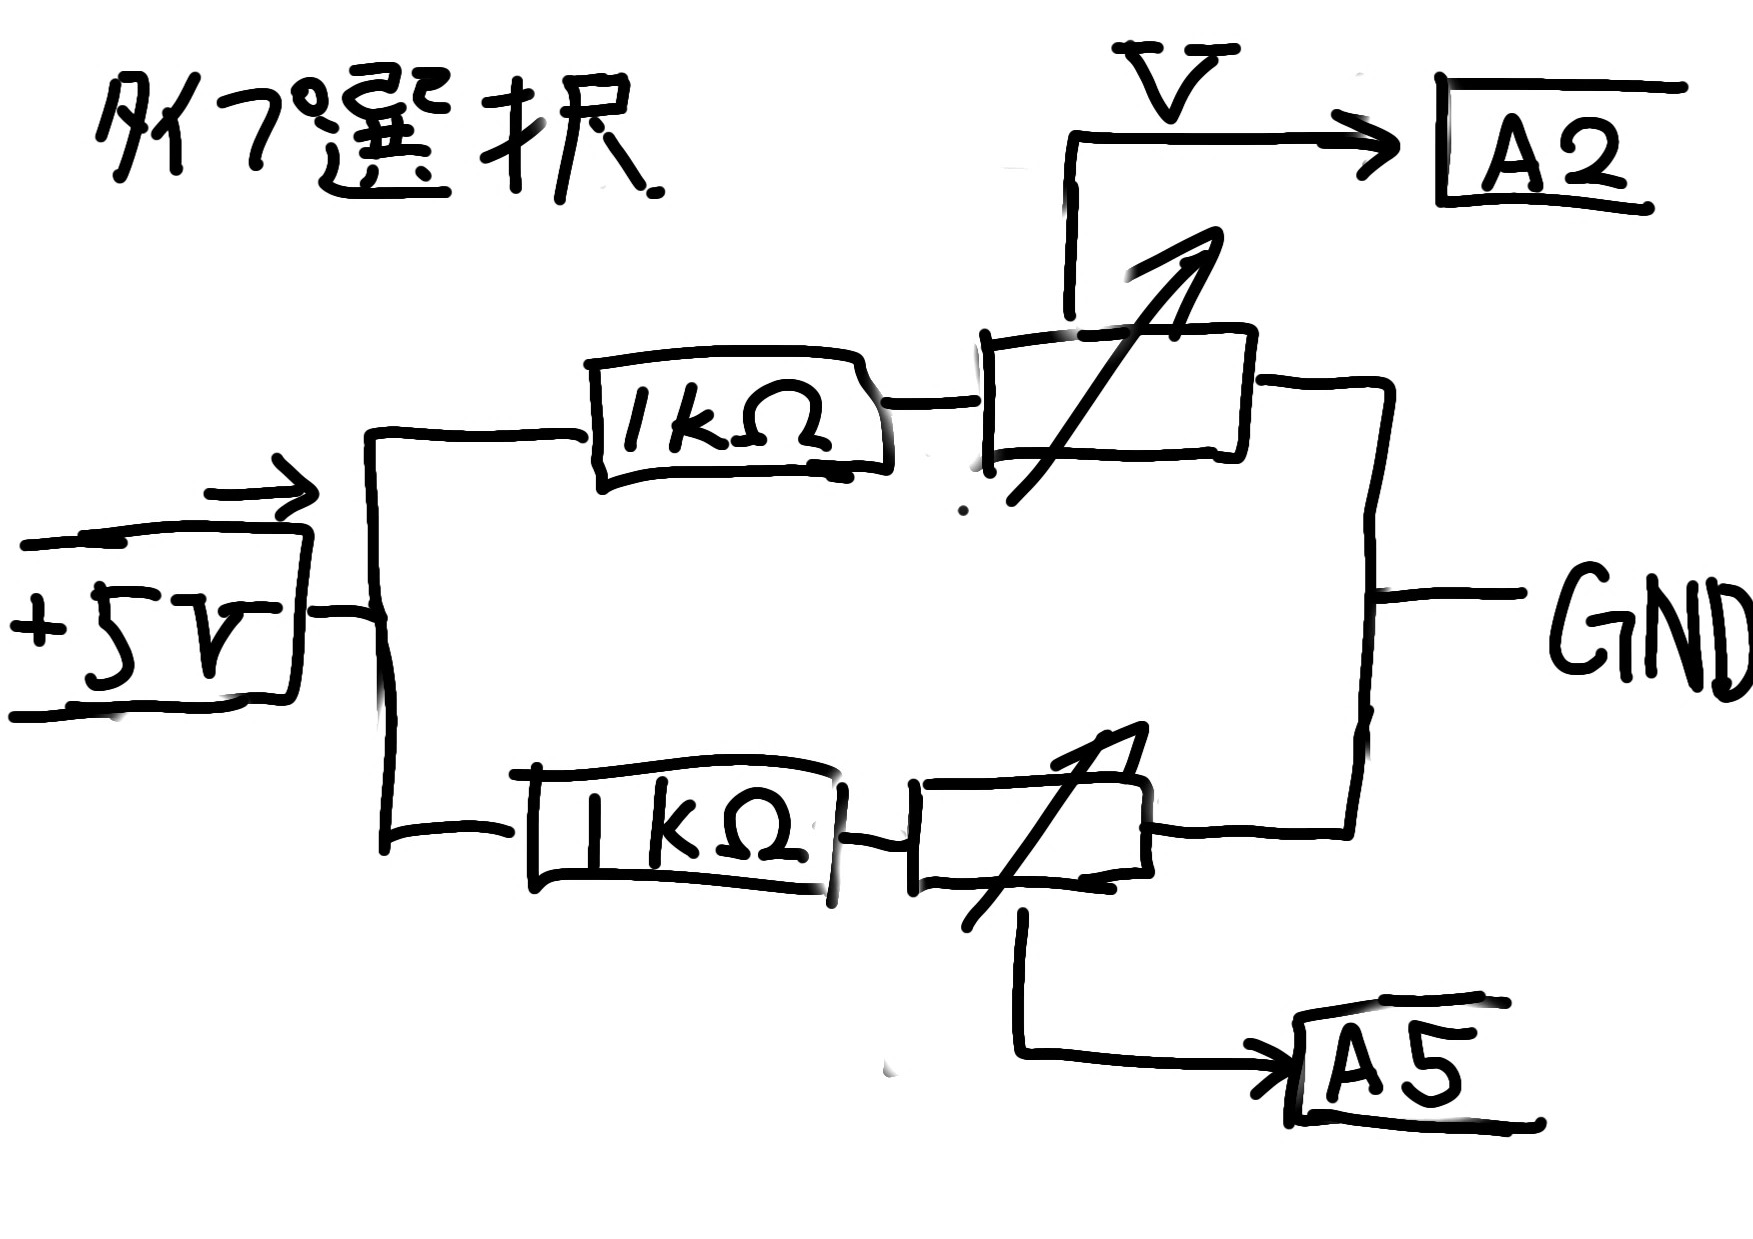
\includegraphics[width=100mm]{typechose.pdf}
    \caption{可変抵抗周辺の回路図}
  \end{center}
\end{figure}
可変抵抗二つを並列に並べることによって、攻撃側、防御側の両方に融通が利くようにし、
またショート防止のために可変抵抗の前に$1k\Omega $の抵抗を直列に配置した。可変抵抗
の抵抗を変化させることによって可変抵抗に流れる電圧、Analog readに流れる電圧を
調整することができる。Anarog readに流れる電圧を$E_{A}$とする。
\begin{figure}[H]
  \begin{center}
    \includegraphics[width=100mm]{typechose_s.pdf}
    \caption{}
  \end{center}
\end{figure}
上の図のように、タイプ選択にもケースストラクチャを利用する。
ケースストラクチャを扱うに当たって、整数に変換すると数値の範囲で条件指定できたので、判定値
$E_{A}\times 100$を計算し、小数点以下切り捨てをした値をケースストラクチャに渡し、その数値に
応じてタイプのString値をタイプ相性判定部分に渡す。
判定値とタイプの関係は以下の表の通りである。原因は解明できなかったが攻撃側と防御側で範囲が異なっていたので
それぞれ載せる。

%%%%表
攻撃側
\begin{tabular}{|c|c|}\hline
  判定値 & タイプ\\ \hline
  0 & Normal \\ \hline
  27 & Fire \\ \hline
  52 & Water \\ \hline
  81 & Grass \\ \hline
  109 & Electric \\ \hline
  138 & Ice \\ \hline
  166 & Fighting \\ \hline
  194 & Poison \\ \hline
  222 & Ground \\ \hline
  250 & Flying \\ \hline
  279 & Psychic \\ \hline
  308 & Bug \\ \hline
  336 & Rock \\ \hline
  364 & Ghost \\ \hline
  392 & Dragon \\ \hline
  420 & Dark \\ \hline
  449 & Steel \\ \hline
  477 & Fairy \\ \hline
\end{tabular}
%%%%表ここまで%%%%%%%%%%

%%%%表%%%%%%%%%%%%%%%
防御側
\begin{tabular}{|c|c|}\hline
  判定値 & タイプ\\ \hline
  0 & Normal \\ \hline
  26 & Fire \\ \hline
  51 & Water \\ \hline
  76 & Grass \\ \hline
  101 & Electric \\ \hline
  126 & Ice \\ \hline
  151 & Fighting \\ \hline
  176 & Poison \\ \hline
  201 & Ground \\ \hline
  226 & Flying \\ \hline
  251 & Psychic \\ \hline
  276 & Bug \\ \hline
  301 & Rock \\ \hline
  326 & Ghost \\ \hline
  351 & Dragon \\ \hline
  376 & Dark \\ \hline
  401 & Steel \\ \hline
  426 & Fairy \\ \hline
\end{tabular}
%%%%表ここまで%%%%%%%%%%%%%

攻撃側の上限は500、防御側の上限は450となっている。
また、フロントパネル上にタイプを表示できるようにもなっている。
\section{実験結果および使い方}
攻撃側、防御側の、可変抵抗を利用したつまみがあるのでそれを回すことでフロントパネル上にタイプが表示される、
もしくはつまみをそのタイプのイラストのところに合わせることでタイプを指定できる。
そうすると組み合わせによってサーボモーターが動き、どのようなダメージ補正がかかるのかを教えてくれる。
例えば下の図では攻撃側がフェアリー、防御側があくにつまみがあっており、ダメージ補正は二倍なので、
サーボモーターも抜群の位置を示している。
\begin{figure}[H]
  \begin{center}
    \includegraphics[width=100mm]{howto.pdf}
    \caption{使用例}
  \end{center}
\end{figure}
また、タイプチェッカーをを使用している様子は以下の動画で確認できる。
\begin{verbatim}
  https://kitaq-my.sharepoint.com/:v:/g/personal/d2531033
_eng_kitakyu-u_ac_jp/Ecgebwzp1sdBqD5P2UWbBWEBd8Iupdlgz10pyelw4KaHCQ?e=ZOdSjB
\end{verbatim}
\section{工夫した点}
最大の工夫した点はタイプの選択をハードウェア上で行えるようにして点である。
この装置を作るにあたってタイプ選択の用紙を自分でibispaintで制作し、可変抵抗に着けたこ
とも工夫の一つといえる。またLEDではなくサーボモーターを用いることで比較的一つの装置でダメージ
効果を表示できた点もいいといえるだろう。またタイプ相性定義でDefaultをうまく利用したことで時短になり、
余った時間をタイプ選択装置の実装に使えたことも工夫によって作品がよくなった一例といえる。
ゲーム性の面では、タイプ相性を予想して当てたり、攻撃側と防御側のタイプを見えないようにして複雑なじゃんけんのような
使い方をすることもできる。また私の友達がやっていたように、私自身のタイプ知識のあら捜しをするのも面白いかもしれない。
しかしタイプ相性表を見ながら確実にやったので無駄な行動であることには間違いない。
\section{考察:計測/制御について学んだこと}
まずオシロスコープの使い方や、テスターの使い方、またどこを計測すればハードウェア上の間違いを見つけやすいか
といったところを学べた。またハードウェアを動かすに当たっては確実な知識と入念な確認が必要なこと。またLabviewの
勉強を通してBool値、Numeric値などの値の種類を確実に把握できるようになり、それを日常の勉強やプログラミングにも
生かせるようになったこと。「ハードウェアのプログラミング」の考え方の初歩、そして制御プログラムの
作成には広い視点も必要だということを学んだ。
\section{感想}
後半の授業が始まったとき、正直壊さないことだけでも頭がいっぱいになっており、ショートしないかどうか
ばかりを考えていた気もする。しかしそのおかげで大きな損傷を電気部品に与えることなくモノづくりをすることが
できた。また最初はつまみでタイプを指定できるようにする計画はもっぱらなく、作っている途中で思いついたものである。
だから実装前は時間が足りなくなるのではないかという風に怖がっていたのだが、面白いものを作りたかったので挑戦した結果、
本当に自分の理想に近いものができてしまったので驚いた。モノづくり全般にいえることであるが、小さいものから作っていき、
それに付け加えたり細かく作りこむことで少しづつ大きなものを作っていくということをこの授業で実践できたので、その貴重な体験を
今後に生かしていきたいと思う。
\begin{thebibliography}{}
  \bibitem{typechart}
 タイプ相性表
  \begin{verbatim}
    http://pokemondb.net/type
  \end{verbatim}
\end{thebibliography}
\end{document}